\chapter{Introduction}
\label{Introduction}
Ravel is an intuitive and powerful way to analyse data. Its key feature is the Ravel: a visual tool for manipulating and analysing data.

This is a blank Ravel---a Ravel with no data attached to it:

\begin{center}
\resizebox{20cm}{!}{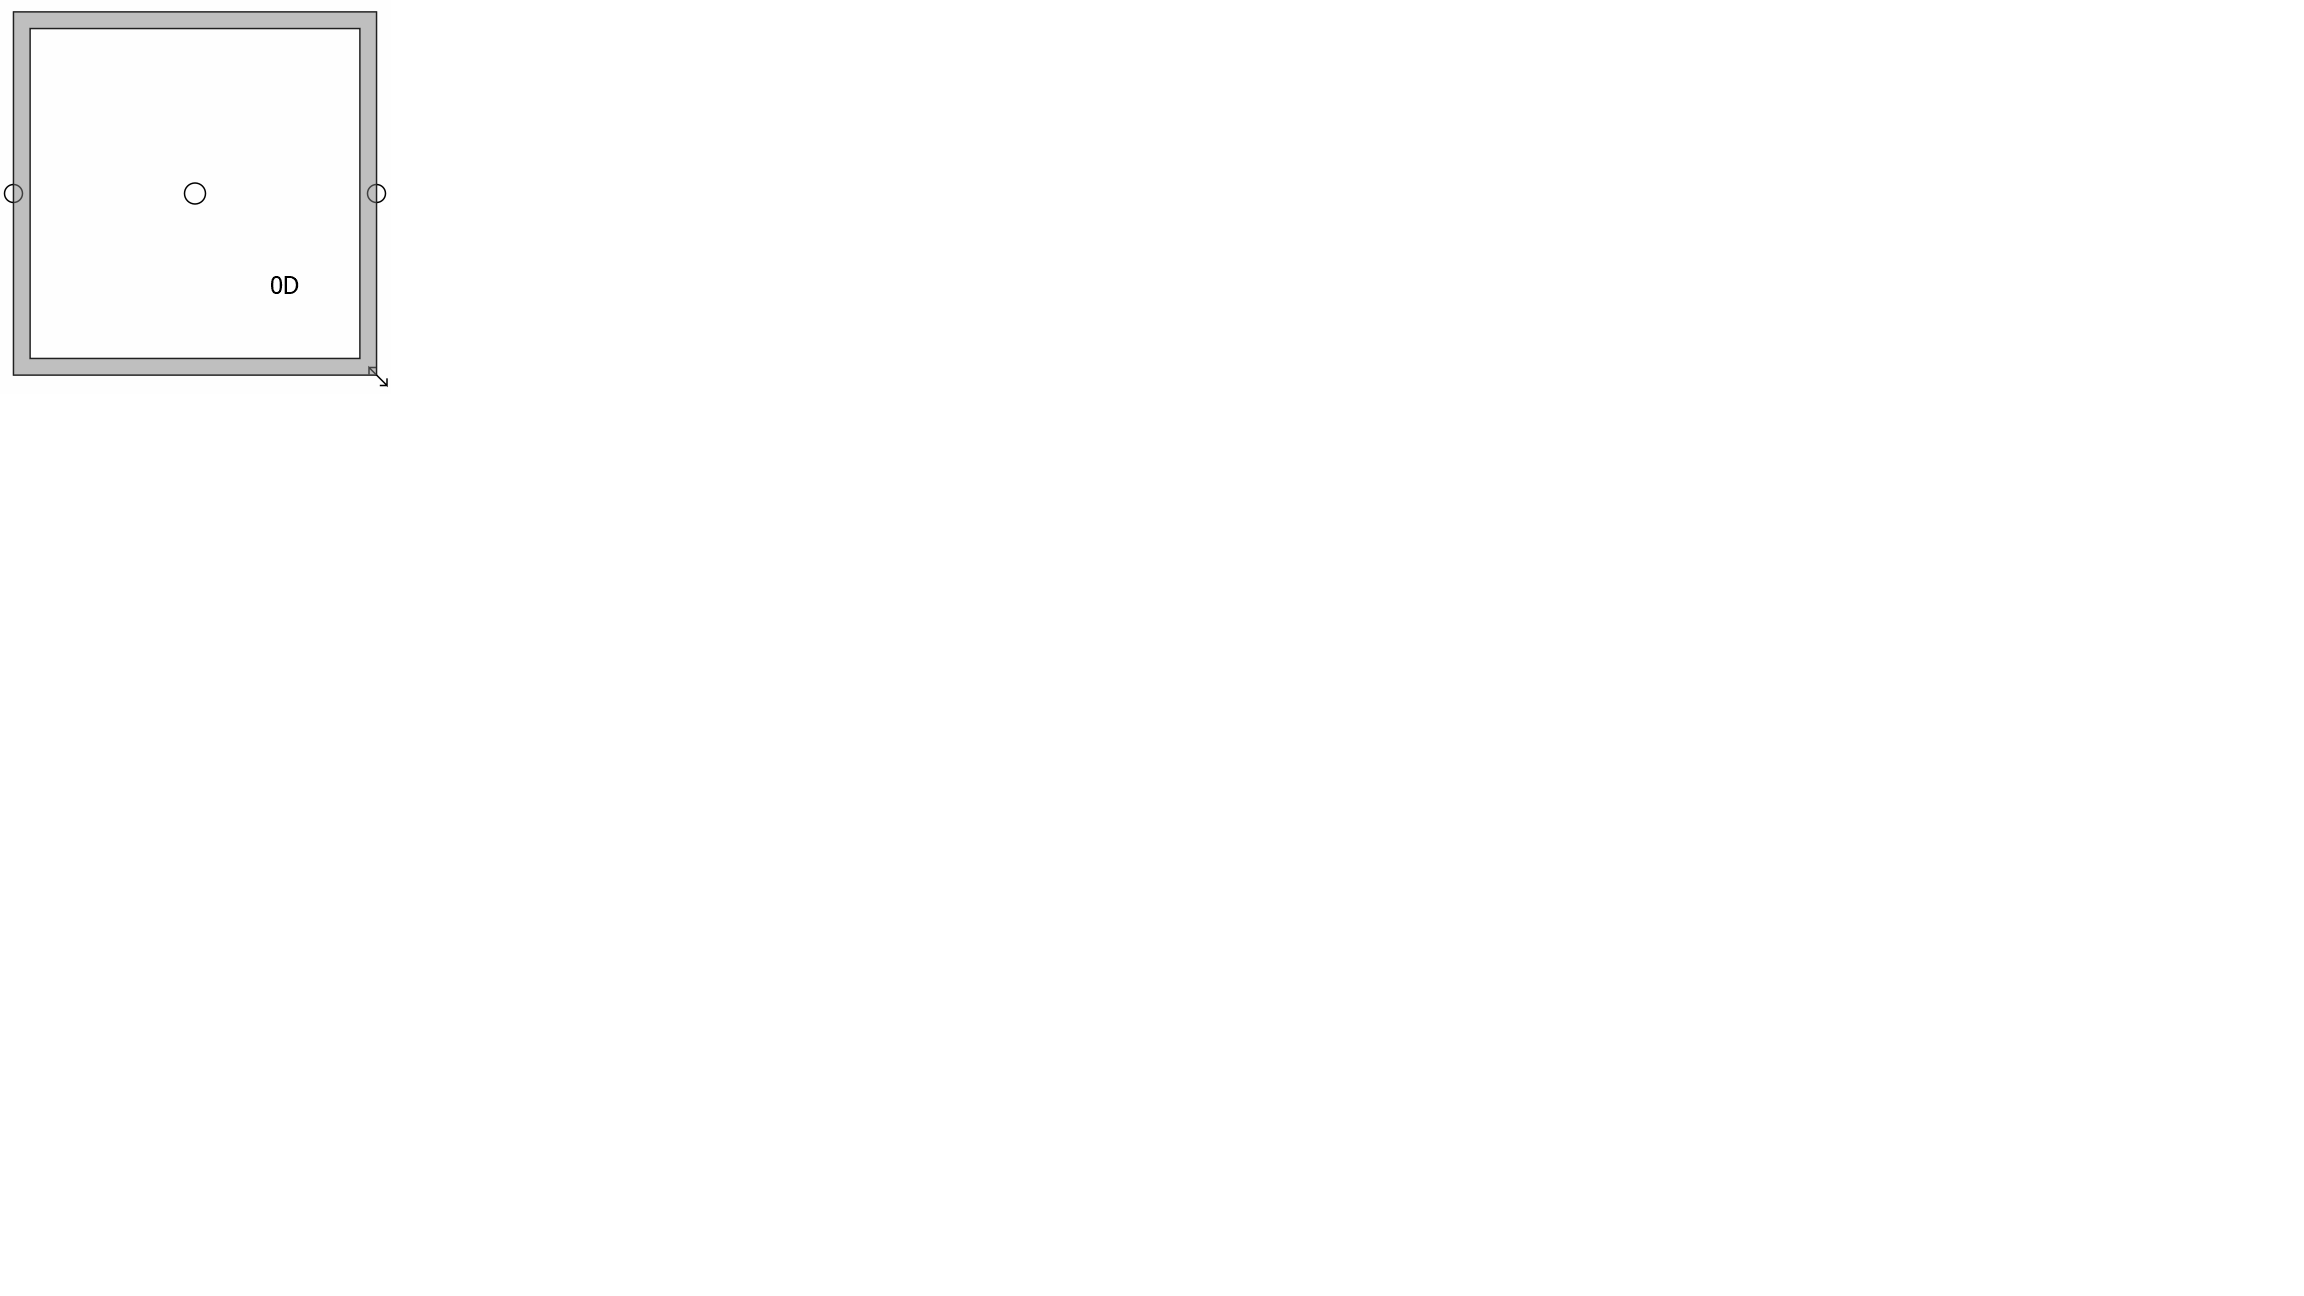
\includegraphics{images/00RavelBlank.png}}
\end{center}

To use a Ravel, you first need to import a data file--at present this must be a CSV file (other data sources will be added in later releases). Once the data is imported, the data object can be attached to a Ravel. This is a Ravel with data attached:

\begin{center}
\includegraphics{images/01RavelDataInflation.eps}
\end{center}

There are many ways to manipulate and display data directly from a Ravel. This is a Ravel with data attached and selected for graphing: the "Year on Year Changes" data is selected from the Unit of Measure axis; two countries (Japan and the United States) are selected from the Reference area axis; Monthly data is chosen from the Frequency axis; and Calipers are applied to the Date axis to select data from 1960 till 2024.

\resizebox{10cm}{!}{\includegraphics{images/01BRavelDataInflationSelected.eps}}

Ravel the object itself makes it far easier to drill down into and visualise data than using either a spreadsheet, or the Pivot Tables that standard Business Intelligence program use.

Ravel the program enables easy analysis of data using self-documenting flowchart formulas.This is a Ravel with data selected--for six countries, on the annualised monthly inflation rate, for dates from January 2001 till January 2024--and assigned to a variable ("Post2000").

\begin{center}
\resizebox{10cm}{!}{\includegraphics{images/02RavelDataInflationGraphed.eps}}
\end{center}

Finally, the data is analyzed by (a) working out the average inflation rate for the selected countries, and (b) subtracting the average from the actual inflation rate for each country.

The average inflation rate was calculated using the formula:

\begin{flushleft}
>
\resizebox{10cm}{!}{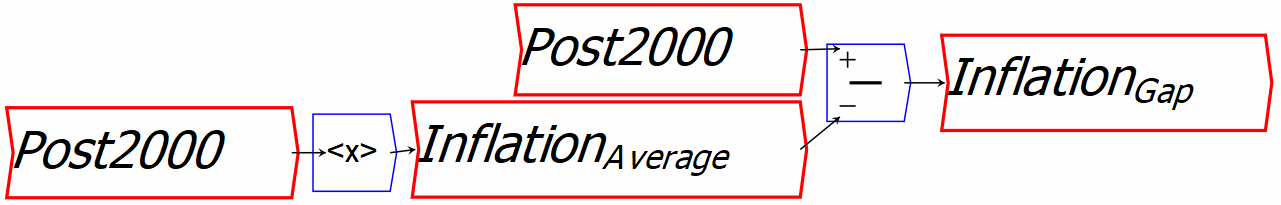
\includegraphics{images/03Formula.png}}
\end{flushleft}

This one formula is applied to every country in the Ravel (six countries in this case) and every quarterly data point (80 quarters). Doing the same analysis with a spreadsheet would require writing an obscure cell reference formula and replicating it across 480 cells.

The final example is the comparison of average inflation outcomes for the six countries, and the deviation of them from the average. This illustrates the capacity of Ravel to rapidly provide insights from data--in this case, that the best-performing country during the post-Covid inflation was Japan, and the worst performing were the USA and UK. This is noteworthy, because both the USA and UK sharply increased interest rates with the intention of reducing inflation, while Japan kept its interest rate constant. Perhaps then, interest rates aren't effective at controlling interest rates?
\begin{center}
\resizebox{10cm}{!}{\includegraphics{images/03RavelDataInflationAnalyzed.eps}}
\end{center}

These examples are drawn from economics, mainly because Ravel's inventor is an economist (and a contrarian one at that). But Ravel can analyze any data you give it---marketing data, scientific data, production data, whatever. It can also handle enormous data sets, far larger than are manageable with Excel.

We hope these examples show how easy it is to turn data into information using Ravel.



